\documentclass[12pt]{article} % 使用 article 文档类,12pt 字体
\usepackage[utf8]{inputenc} % 支持 UTF-8 编码
\usepackage{amsmath} % 提供高级数学环境和符号
\usepackage{amssymb} % 提供更多数学符号,如 \mathbb{R}
\usepackage{braket}  % 用于量子力学中的 ket|>, bra<|, braket 符号
\usepackage{graphicx} % 用于插入图片 (此处为图1的占位符)
\usepackage[margin=1in]{geometry} % 设置页边距为1英寸
\usepackage[T1]{fontenc} % 提高字体质量和编码一致性
\usepackage{tikz} % 用于绘制图形
\usetikzlibrary{decorations.pathreplacing} % 修复 TikZ brace 装饰错误

% 设置标题和日期信息
\title{Homework 5}
\author{Zheng Xiaoyang \\ SID: 3035204227}
\date{C191A: Introduction to Quantum Computing, Fall 2025 \\ Due: Monday, Oct. 6 2025, 10:00 pm}
\begin{document}

\maketitle % 生成标题

\section{Grover Search}

In this question, we'll try to get a geometric understanding of Grover's algorithm. Note that this analysis is a recap of material from lecture.

Recall that in Grover's algorithm we have some distinguished, marked element \(a \in \{1, \dots, N\} = [N]\) and have access to some function \(f : [N] \to \{0,1\}\) that recognizes \(a\), i.e., \(f(a) = 1\) and \(f(x) = 0\) if \(x \ne a\). Our goal is to use \(f\) to find \(a\).

Let \(\ket{a}\) be the standard basis state labeled with \(a\), and define the uniform superposition over unmarked elements:
\[ \ket{e} = \frac{1}{\sqrt{N-1}} \sum_{x \in [N] \text{ and } x \ne a} \ket{x}. \]
At all times, we will maintain a quantum state in the two-dimensional subspace spanned by \(\ket{a}\) and \(\ket{e}\). That is, our state can be written as \(\alpha \ket{a} + \beta \ket{e}\) (\(\alpha, \beta \in \mathbb{R}\)) and therefore we can understand the algorithm in a two dimensional space.

\subsection{}
We start with the state \(\ket{u} = \frac{1}{\sqrt{N}} \sum_{x \in [N]} \ket{x}\). Express \(\ket{u}\) in terms of \(\ket{a}\) and \(\ket{e}\). What is the angle \(\theta\) between \(\ket{u}\) and \(\ket{e}\) in the two dimensional space in Fig. 1?
\subsubsection*{Solution}
\[\ket{u} = \frac{1}{\sqrt{N}} \ket{a} + \sqrt{\frac{N-1}{N}} \ket{e}\]
The angle \(\theta\) between \(\ket{u}\) and \(\ket{e}\) is given by:
\[\cos(\theta) = \braket{e|u} = \sqrt{\frac{N-1}{N}}\]
Thus,
\[\theta = \cos^{-1}\left(\sqrt{\frac{N-1}{N}}\right)\] 
\subsection{}
Apply the oracle \(U_f\) (defined as \(U_f\ket{x} = (-1)^{f(x)}\ket{x}\)) to \(\ket{u}\), obtaining the state \(\ket{\psi}\). Draw \(\ket{\psi}\) in the above two dimensional space.
\subsubsection*{Solution}
\[\ket{\psi} = U_f \ket{u} = \frac{1}{\sqrt{N}} \ket{a} - \sqrt{\frac{N-1}{N}} \ket{e}\]
This operation reflects \(\ket{u}\) about the axis orthogonal to \(\ket{a}\), resulting in the state \(\ket{\psi}\).

\subsection{}
Consider the matrix \(2 \ket{u}\bra{u} - I\). Prove that it is unitary.
\subsubsection*{Solution}
To prove that \(2 \ket{u}\bra{u} - I\) is unitary, we need to show that:
\[(2 \ket{u}\bra{u} - I)(2 \ket{u}\bra{u} - I)^\dagger = I\]
Calculating the left-hand side:
\[(2 \ket{u}\bra{u} - I)(2 \ket{u}\bra{u} - I) = 4 \ket{u}\bra{u}\ket{u}\bra{u} - 2 \ket{u}\bra{u} - 2 \ket{u}\bra{u} + I\]
Since \(\bra{u}\ket{u} = 1\), we have:
\[= 4 \ket{u}\bra{u} - 4 \ket{u}\bra{u} + I = I\]
Thus, \(2 \ket{u}\bra{u} - I\) is unitary.
\begin{figure}[h]
    \centering
    % 用 TikZ 绘制 Grover 算法二维子空间
    \begin{tikzpicture}[scale=2,>=stealth]
        % 坐标轴
        \draw[->] (0,0) -- (1.2,0) node[right] {$\ket{e}$};
        \draw[->] (0,0) -- (0,1.2) node[above] {$\ket{a}$};
        % |u| 向量
        \draw[->,thick,blue] (0,0) -- (0.45,0.89) node[above right] {$\ket{u}$};
        % |ψ| 向量
        \draw[->,thick,red] (0,0) -- (0.45,-0.89) node[below right] {$\ket{\psi}$};
        % 角度 θ
        \draw [->] (0.3,0) arc (0:63.4:0.3);
        \node at (0.38,0.18) {$\theta$};
        % 辅助虚线
        \draw[dashed,gray] (0.45,0.89) -- (0.45,0);
        \draw[dashed,gray] (0.45,-0.89) -- (0.45,0);
    \end{tikzpicture}
    \caption{The two-dimensional subspace spanned by $\ket{a}$ and $\ket{e}$, showing $\ket{u}$ and $U_f\ket{u} = \ket{\psi}$.}
    \label{fig:subspace}
\end{figure}

\subsection{}
Discuss how to implement the unitary operation \(2\ket{u}\bra{u} - I\) using 2-qubit gates.
\subsubsection*{Solution}
To implement the unitary operation \(2\ket{u}\bra{u} - I\) using 2-qubit gates, we can follow these steps:
\begin{enumerate}
    \item Prepare the state \(\ket{u}\) using Hadamard gates on all qubits.
    \item Use a series of controlled-NOT (CNOT) gates to create the reflection about \(\ket{u}\). This involves creating an ancilla qubit that is flipped if the state is \(\ket{u}\).
    \item Apply a phase flip (Z gate) to the ancilla qubit.
    \item Reverse the CNOT operations to disentangle the ancilla qubit.
    \item Finally, apply Hadamard gates again to return to the original basis.
\end{enumerate}

\begin{figure}[h]
    \centering
    % 美化后的 2-qubit Grover diffusion operator circuit
    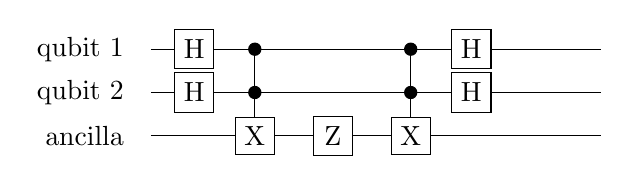
\begin{tikzpicture}[scale=1.1, quantum/.style={draw,minimum size=0.5cm,fill=white}]
        % 线路位置
        \def\yA{1.2}
        \def\yB{0.7}
        \def\yC{0.2}
        % 线路长度
        \def\xstart{0}
        \def\xend{5.2}
        % 标签
        \node[left] at (\xstart-0.2,\yA) {qubit 1};
        \node[left] at (\xstart-0.2,\yB) {qubit 2};
        \node[left] at (\xstart-0.2,\yC) {ancilla};
        % 水平线
        \draw (\xstart,\yA) -- (\xend,\yA);
        \draw (\xstart,\yB) -- (\xend,\yB);
        \draw (\xstart,\yC) -- (\xend,\yC);
        % H 门
        \node[quantum] (h1) at (0.5,\yA) {H};
        \node[quantum] (h2) at (0.5,\yB) {H};
        % 控制-X
        \draw (1.2,\yA) -- (1.2,\yC);
        \filldraw (1.2,\yA) circle (2pt);
        \filldraw (1.2,\yB) circle (2pt);
        \node[quantum,minimum size=0.35cm] (x1) at (1.2,\yC) {X};
        % Z 门
        \node[quantum] (z) at (2.1,\yC) {Z};
        % 反向控制-X
        \draw (3.0,\yA) -- (3.0,\yC);
        \filldraw (3.0,\yA) circle (2pt);
        \filldraw (3.0,\yB) circle (2pt);
        \node[quantum,minimum size=0.35cm] (x2) at (3.0,\yC) {X};
        % 末尾 H 门
        \node[quantum] (h3) at (3.7,\yA) {H};
        \node[quantum] (h4) at (3.7,\yB) {H};
    \end{tikzpicture}
    \caption{Diffusion operator circuit: implements the reflection \(2\ket{u}\bra{u} - I\) on two qubits using Hadamard, CNOT, ancilla, and phase flip.}
    \label{fig:grover-circuit}
\end{figure}

\subsection{}
Apply the unitary \(2\ket{u}\bra{u} - I\) to the state \(\ket{\psi}\). Draw the resulting state in the above two dimensional space. What operation is it performing on this space?
\subsubsection*{Solution}
Applying the unitary \(2\ket{u}\bra{u} - I\) to the state \(\ket{\psi}\):
\[\ket{\phi} = (2\ket{u}\bra{u} - I)\ket{\psi}\]
This operation reflects \(\ket{\psi}\) about the axis defined by \(\ket{u}\), resulting in the state \(\ket{\phi}\). In the two-dimensional space, this operation effectively rotates the state closer to \(\ket{a}\).  

\subsection{}
Apply the operation \((2\ket{u}\bra{u} - I)U_f\) two more times on the resulting state from 1.5 and draw the two resulting states in the above two dimensional space. What angle of rotation does \((2\ket{u}\bra{u} - I)U_f\) perform in the space?
\subsubsection*{Solution}
Each application of \((2\ket{u}\bra{u} - I)U_f\) rotates the state by an angle of \(2\theta\) towards \(\ket{a}\). After two more applications, the total rotation from the initial state \(\ket{u}\) is \(5\theta\). The resulting states can be drawn in the two-dimensional space, showing the progressive rotation towards \(\ket{a}\).

\subsection{}
Grover's algorithm repeatedly applies \((2\ket{u}\bra{u} - I)U_f\) to \(\ket{u}\) to get close to \(\ket{a}\). How many times should you apply this operation to get closest to the state \(\ket{a}\)?
\noindent Hint: Use the small angle approximation \(\sin(\theta) \approx \theta\).
\subsubsection*{Solution}
To get closest to the state \(\ket{a}\), we want to maximize the overlap with \(\ket{a}\). The angle between \(\ket{u}\) and \(\ket{a}\) is \(\frac{\pi}{2} - \theta\). Each application of \((2\ket{u}\bra{u} - I)U_f\) rotates the state by \(2\theta\). We want to find \(k\) such that:
\[(2k + 1)\theta \approx \frac{\pi}{2}\]
Using the small angle approximation \(\sin(\theta) \approx \theta\), we have:
\[k \approx \frac{\pi}{4\theta} - \frac{1}{2}\]
Since \(\theta \approx \frac{1}{\sqrt{N}}\) for large \(N\), we get:
\[k \approx \frac{\pi}{4} \sqrt{N} - \frac{1}{2}\]
Thus, the number of applications needed is approximately \(\frac{\pi}{4} \sqrt{N}\).

\section{Shor's Factoring Algorithm}

In this question, we will go through a small example of Shor's factoring algorithm. Recall the following facts about the quantum Fourier transform (\(\text{QFT}_M\)) applied to periodic and shifted states:

\begin{enumerate}
    \item QFT on periodic states: Let \(1 < r < M\) be an integer that divides \(M\). Then,
    \begin{align}
        &\text{QFT}_M \left( \frac{1}{\sqrt{r}} (\ket{0} + \ket{r} + \ket{2r} + \dots + \ket{M-r})) \right) \\ &= \frac{1}{\sqrt{r}} (\ket{0} + \ket{M/r} + \ket{2M/r} + \dots + \ket{(r-1)M/r})) \label{eq:qft_periodic}
    \end{align}
    \item QFT on shifted states: If \(\ket{\psi} = \sum_{k=0}^{M-1} \alpha_k \ket{k}\) and \(\ket{\psi+t} = \sum_{k=0}^{M-1} \alpha_k \ket{k+t \bmod N})\), then \(\text{QFT}_M\) applied to the two states are related by: If
    \begin{equation} \label{eq:qft_psi}
        \text{QFT}_M \ket{\psi} = \sum_{k=0}^{M-1} \beta_k \ket{k},
    \end{equation}
    then
    \[ \text{QFT}_M \ket{\psi+t} = \sum_{k=0}^{M-1} \omega^{kt} \beta_k \ket{k}. \]
\end{enumerate}

We will work through an example of factoring \(N = 21\) using \(\text{QFT}_M\) with \(M = 12\).

\subsection{}
Let \(a = 2\). Calculate the state \(\ket{\psi} = \frac{1}{\sqrt{M}} \sum_{x=0}^{M-1} \ket{x} \ket{a^x \bmod N}\).
\subsubsection*{Solution}
Calculating \(a^x \bmod N\) for \(x = 0, 1, \dots, 11\):
\begin{align*}
    2^0 \bmod 21 &= 1 ; 2^1 \bmod 21 = 2 ; 2^2 \bmod 21 = 4 \\
    2^3 \bmod 21 &= 8 ; 2^4 \bmod 21 = 16 ; 2^5 \bmod 21 = 11 \\
    2^6 \bmod 21 &= 1 ; 2^7 \bmod 21 = 2 ; 2^8 \bmod 21 = 4 \\
    2^8 \bmod 21 &= 4 ; 2^9 \bmod 21 = 8 ; 2^{10} \bmod 21 = 16 \\
    2^{11} \bmod 21 &= 11
\end{align*}
Thus, the state \(\ket{\psi}\) is:
\[\ket{\psi} = \frac{1}{\sqrt{12}} \sum_{x=0}^{11} \ket{x} \ket{a^x \bmod N} \]

\subsection{}
Suppose we measure the second register of \(\ket{\psi}\) and obtain "1". What is the resulting state on the first register? Then perform \(\text{QFT}_M\) on the first register. What is the resulting state on the first register? Now measure this state in the standard basis. What are the possible measurement outcomes?
\subsubsection*{Solution}
After measuring the second register and obtaining "1", the first register collapses to the superposition of states corresponding to \(x\) values where \(a^x \bmod N = 1\). From the calculations above, this occurs at \(x = 0, 6\). Thus, the resulting state on the first register is:
\[\ket{\psi_1} = \frac{1}{\sqrt{2}} (\ket{0} + \ket{6})\]
Now, applying \(\text{QFT}_M\) to \(\ket{\psi_1}\):
\[\text{QFT}_M \ket{\psi_1} = \frac{1}{\sqrt{2}} \left( \text{QFT}_M \ket{0} + \text{QFT}_M \ket{6} \right)\]
Using the QFT definition, we have:
\[\text{QFT}_M \ket{0} = \frac{1}{\sqrt{12}} \sum_{k=0}^{11} \ket{k}\]
\[\text{QFT}_M \ket{6} = \frac{1}{\sqrt{12}} \sum_{k=0}^{11} e^{2\pi i \cdot 6k/12} \ket{k} = \frac{1}{\sqrt{12}} \sum_{k=0}^{11} (-1)^k \ket{k}\]
Combining these, we get:
\[\text{QFT}_M \ket{\psi_1} = \frac{1}{\sqrt{24}} \sum_{k=0}^{11} (1 + (-1)^k) \ket{k} = \frac{1}{\sqrt{6}} (\ket{0} + \ket{2} + \ket{4} + \ket{6} + \ket{8} + \ket{10})\]
The possible measurement outcomes are \(0, 2, 4, 6, 8, 10\).
\subsection{}
Suppose we repeat the above experiment, now the first step (when measuring the second register) gives "4". Answer the same questions as above.
\subsubsection*{Solution}
After measuring the second register and obtaining "4", the first register collapses to the superposition of states corresponding to \(x\) values where \(a^x \bmod N = 4\). From the calculations above, this occurs at \(x = 2, 8\). Thus, the resulting state on the first register is:
\[\ket{\psi_2} = \frac{1}{\sqrt{2}} (\ket{2} + \ket{8})\]
Now, applying \(\text{QFT}_M\) to \(\ket{\psi_2}\):
\[\text{QFT}_M \ket{\psi_2} = \frac{1}{\sqrt{2}} \left( \text{QFT}_M \ket{2} + \text{QFT}_M \ket{8} \right)\]
Using the QFT definition, we have:
\[\text{QFT}_M \ket{2} = \frac{1}{\sqrt{12}} \sum_{k=0}^{11} e^{2\pi i \cdot 2k/12} \ket{k}\]
\[\text{QFT}_M \ket{8} = \frac{1}{\sqrt{12}} \sum_{k=0}^{11} e^{2\pi i \cdot 8k/12} \ket{k}\]
Combining these, we get:
\[\text{QFT}_M \ket{\psi_2} = \frac{1}{\sqrt{24}} \sum_{k=0}^{11} (e^{2\pi i \cdot 2k/12} + e^{2\pi i \cdot 8k/12}) \ket{k}\]
The possible measurement outcomes can be calculated from the resulting state, which will yield a distribution over the basis states. The possible measurement outcomes are \(0, 3, 6, 9\).
\subsection{}
Suppose we repeat the above experiment 4 times in total. Each time we record a measurement outcome of the first register (after performing \(\text{QFT}_M\)). Suppose the recorded outcomes are all different. What is their greatest common divisor \(g\)?
\subsubsection*{Solution}
Assuming the recorded outcomes from the four experiments are \(x_1, x_2, x_3, x_4\), we can calculate their greatest common divisor \(g\) using the Euclidean algorithm. For example, if the outcomes are \(0, 2, 4, 6\), then:
\[g = \text{gcd}(0, 2, 4, 6) = 2\]
The actual value of \(g\) will depend on the specific outcomes obtained from the experiments.  

\subsection{}
Calculate \(\text{gcd}(N, a^{M/2g} - 1)\) and \(\text{gcd}(N, a^{M/2g} + 1)\). Are they prime factors of \(N\)?
\subsubsection*{Solution}
Given \(N = 21\), \(a = 2\), \(M = 12\), and \(g = 2\) (from the previous example), we calculate:
\[a^{M/2g} = 2^{12/4} = 2^3 = 8\]
Now, we compute:
\[\text{gcd}(21, 8 - 1) = \text{gcd}(21, 7) = 7\]
\[\text{gcd}(21, 8 + 1) = \text{gcd}(21, 9) = 3\]
Both \(7\) and \(3\) are prime factors of \(N = 21\).
\end{document}
\end{document}
